\subsection{Installation initiale des NAS}

\begin{important}
Les opérations d'installation initiale doivent être réalisées sur les deux NAS.
\end{important}

Les NAS sont détectables à l'aide de l'outil Synology Assistant\footnote{\url{https://kb.synology.com/fr-fr/DSM/help/Assistant/assistant}}.\\

\begin{tip}
Les NAS sont supposés non-configurés.
\end{tip}

Une fois l'adresse IP identifiée, se connecter au NAS à l'aide d'un navigateur web. Le wizard d'installation se lance automatiquement.\\
\begin{enumerate}
    \item Lancer l'assistant d'installation (figure \ref{fig:03-wizard-01})
    \item Si un accès à Internet est disponible, télécharger la dernière version de DSM (figure \ref{fig:03-wizard-02})
    \item Le NAS récupère la mise à jour, l'applique et redémarre automatiquement
    \item Le NAS installe et exécute automatiquement les paquets élémentaires (en cas d'installation sans accès à Internet, ces paquets devront être téléchargés manuellement)
    \item Le NAS affiche un nouvel écran d'accueil (figure \ref{fig:03-wizard-03})
    \item Définnir le nom d'hôte et le compte d'administration initial (figure \ref{fig:03-wizard-04})
    \item Définir le mode de mises à jour du NAS (figure \ref{fig:03-wizard-05})
    \item L'installation initiale est terminée
\end{enumerate}

\begin{figure}[H]
    \centering
    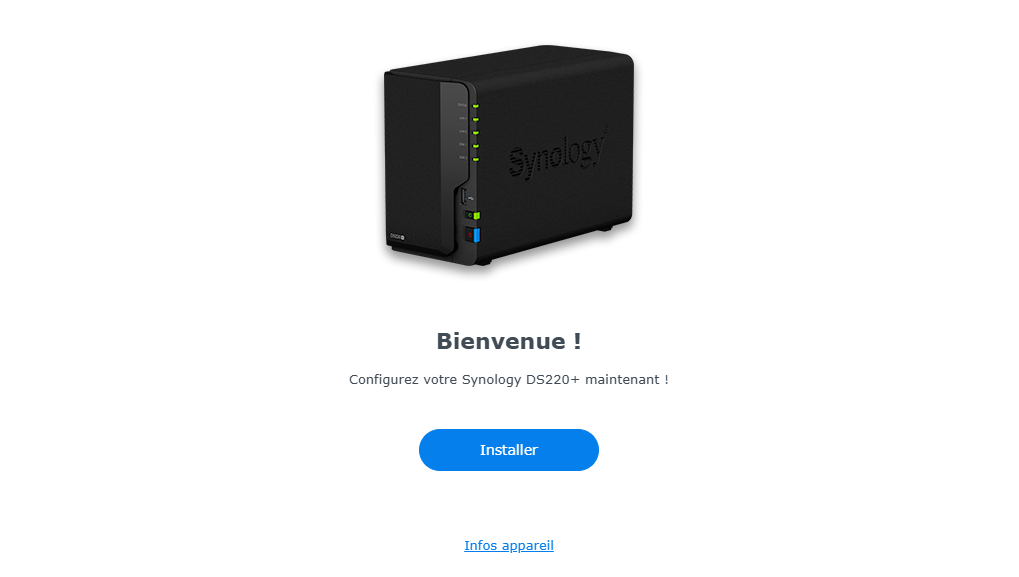
\includegraphics[width=1.0\textwidth]{03-Storage-config.tex/Images/03-wizard-01.png}
    \caption{NAS - Installation - Wizard - Accueil}
    \label{fig:03-wizard-01}
\end{figure}

\begin{figure}[H]
    \centering
    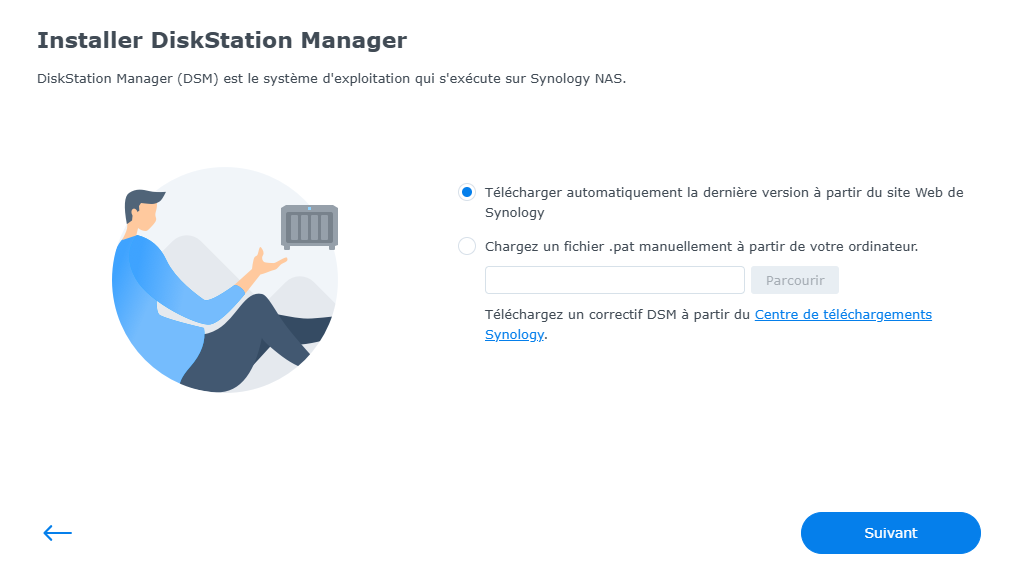
\includegraphics[width=1.0\textwidth]{03-Storage-config.tex/Images/03-wizard-02.png}
    \caption{NAS - Installation - Wizard - Source de mise à jour}
    \label{fig:03-wizard-02}
\end{figure}

\begin{figure}[H]
    \centering
    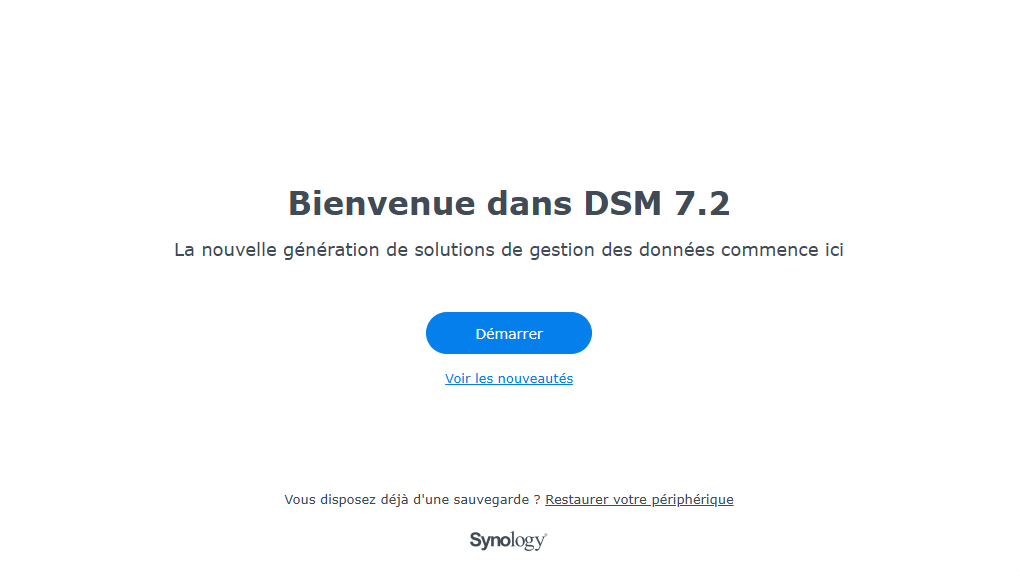
\includegraphics[width=1.0\textwidth]{03-Storage-config.tex/Images/03-wizard-03.png}
    \caption{NAS - Installation - Wizard - Nouvel accueil}
    \label{fig:03-wizard-03}
\end{figure}

\begin{figure}[H]
    \centering
    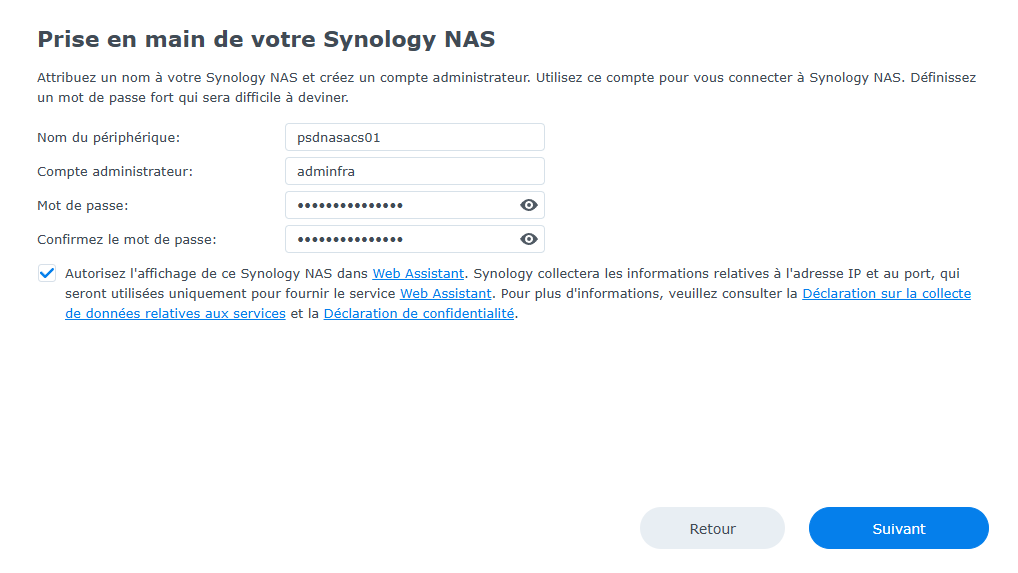
\includegraphics[width=1.0\textwidth]{03-Storage-config.tex/Images/03-wizard-04.png}
    \caption{NAS - Installation - Wizard - Nom d'hôte et compte d'administration}
    \label{fig:03-wizard-04}
\end{figure}

\begin{figure}[H]
    \centering
    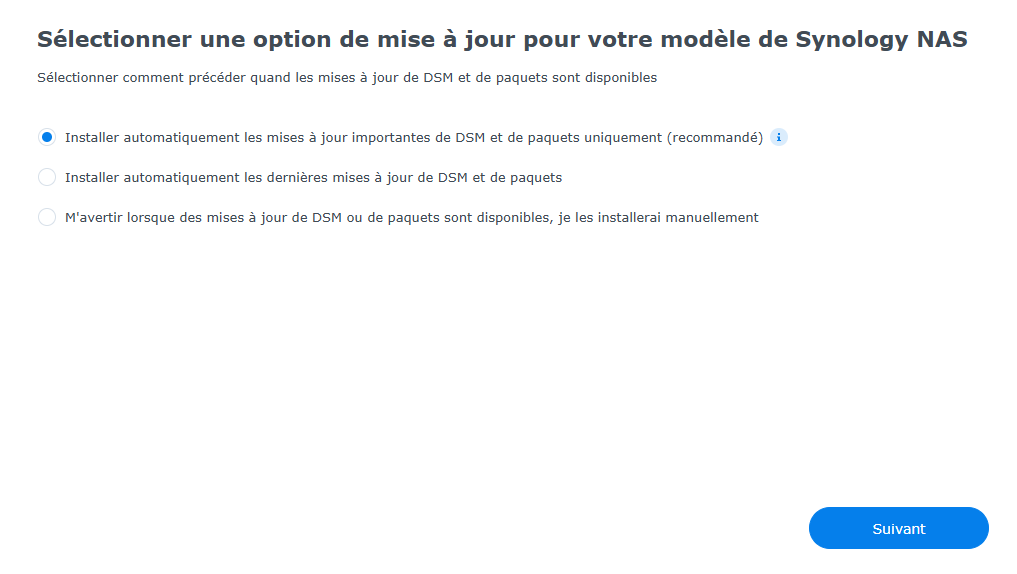
\includegraphics[width=1.0\textwidth]{03-Storage-config.tex/Images/03-wizard-05.png}
    \caption{NAS - Installation - Wizard - Mises à jour}
    \label{fig:03-wizard-05}
\end{figure}
